\chapter{TonePrint}
\label{TonePrintConcept}

The purpose of this chapter is to give the reader a understanding of what the TonePrint concept is and how it works. In this cahpter there will be a description of what a TonePrint is and how it is created with TC Electronics software. The information in this chapter could be essential to understand the later thoughts and considerations, regarding the development of a TonePrint community.
%This chapter works as a in depth description of the TonePrint Concept. This information in this chapter could be essential to understand the later thoughts and considerations, regarding the development of a TonePrint community.

\section{What is TonePrint?}
\label{WhatIsTonePrint}

Effect pedals is a normal piece of equipment used by guitarists and bassists, in many different music genres. An effect pedal works by changing the input signal from the instrument, accordingly to the effect type. This gives the musician the ability to change the sound of his or hers instrument, with a simple push on a button. By using normal effect pedals, you're normally limited in the sense of only being able to adjust a small number of parameters on physical knobs on the pedal. A simple guitar pedal is shown on \autoref{fig:EffectPedalExample}. On this example there is three separately adjustable parameters on the pedal (Dwell, Mix and Tone), which each have its own knob. This limits the range of different sounds, which a pedal enables the user to create. In 2011 TC Electronics wanted to get rid of this limitation so they created the TonePrint concept.\\
A Pedal containing the TonePrint technology enables the users to change the sound of the pedal, beyond the parameters presented by the physical knobs. Using the TonePrint application the users can transfer a range of different premade variations of the effect, directly to the pedal. These premade variations is called TonePrints. In collaboration with multiple famous guitarists and bas players have TC Electronics create TonePrints for a number of pedals used by the artists them selves \parencite{PDF:TonePrintAnalyse}. The TonePrints are created by tweaking all the parameters which are able for the given pedal, which isn't just the ones that are represented by the physical knobs. When the creators of the TonePrint is satisfied with the result is the TonePrint uploaded to the TonePrint library, enabling every one with a pedal of the same type the TonePrint was designed fore, to download the TonePrint and use the effect to sound just like the artist whom created it. The TonePrints created together with famous musicians will from now on be referred to as "\textbf{Artist TonePrints}". \\
Due to requests from the TonePrint users did TC Electronic in ?? launch what we will refer to as "\textbf{User TonePrints}". The main difference between Artist- and User TonePrints is the creator of the TonePrint. A User TonePrint is a TonePrint which is created by a user, using the either the TonePrint smartphone application or the computer software "TonePrint Editor"(Editor manual som kilde). With User TonePrints does the user of a TonePrint pedal have he opportunity to alter all the different parameters for the effect, making the sound just as he or she desires.(Det skal måske rettes så det ikke ser ud til at Appen og editoren er noget forskelligt, for det tror jeg ikke det er.)


\begin{figure}[H]
	\centering
	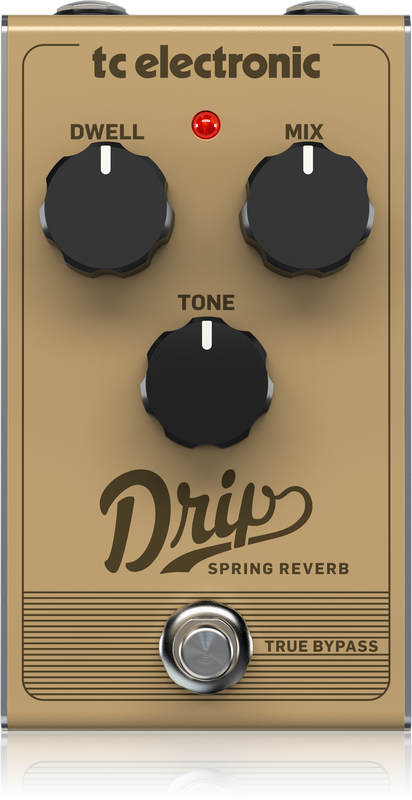
\includegraphics[width=.20\textwidth]{Graphics/EffectPedalExample}
	 \caption{This figure shows a Drip spring reverb effect pedal by TC Electronics \url{https://www.tcelectronic.com/Categories/Tcelectronic/Guitar/Stompboxes/DRIP-SPRING-REVERB/p/P0CQ2\#googtrans(en|en)}.}
    \label{fig:EffectPedalExample}
\end{figure}

\section{TonePrint software}
\label{TonePrintSoftware}
As mentioned in \autoref{WhatIsTonePrint} is a key item for the TonePrint concept, the software in either the smartphone app or the computer software. It is from these softwares the users are able to brows the different Artist TonePrints and create their own User TonePrints. \\
When wanting to use a Artist TonePrint, the user have different options. Either the user can chose to brows the library by the artist whom have co-created the TonePrint, or by brows by the different TonePrint pedals, as shown on \autoref{fig:BrowsByPedal}. Both ways the users is still given the information of which artist and pedal type. When a user has found the desired Artist TonePrint there is two ways of transferring it to the pedal. This can be done by either using a cable connection between the computer or smartphone and the pedal. The other way is to send a sound signal from the TonePrint app through the pickups on the instrument to the pedal, this is called "beaming".


\begin{figure}[H]
	\centering
	
\includegraphics[width=.20\textwidth]{Graphics/Placeholder}
	 \caption{Here its illustrated how a user can select a Artist TonePrint by browsing the TonePrint Pedals.}
    \label{fig:BrowsByPedal}
\end{figure}

when wanting to create a User TonePrint the user can either use the smartpone app or the computer software, which doesn't differ in capability, only the interface. Firstly the user have to connect the computer or phone with the pedal with a cable, whereafter the editor features will appear. The users than has the option to change the parameters with the help of sliders and buttons on the interface. The user can also assign other parameters to the buttons on the pedal, than the ones that is the default. 


\begin{itemize}
  \item What is TonePrint
  \begin{itemize}
    \item How do regular pedals work?
    \item What is special about TonePrint?
    \item What is Artist TonePrint?
    \item What is User TonePrint and what does it mean.
  \end{itemize}
  \item The TonePrint editor
  \begin{itemize}
    \item How does the Editor work (Just the basic principles)?
    \item The use of the App (Beaming, editing)
  \end{itemize}
  \item Shall we mention the lack of platform?
\end{itemize}


%\begin{figure}[H]
%	\centering
%	\includegraphics[resolution=300,scale=1]{}
%	\caption{}
%	\label{fig:}
%\end{figure}
%\noindent



%In 2011 TC Electronic revealed their first TonePrint pedals, opening a new playground for musicians and tone tweakers. By applying the smartphone as tool for setting the desired parameters for an effect type, the user can beam a preset from his or her smartphone directly to the pedal holding the effect type in question. The number of parameters varies between pedal types, and each setting of these parameters is what is simply referred to as \textit{TonePrints} \parencite{WEB:AboutTonePrints}.

%TC Electronic's application holds multiple templates made in-house with different effect types and styles, but it also holds multiple TonePrints created in collaboration with famous guitarists. These presets are referred to as \textit{Artist TonePrints}, and the expectation is that the user will have a clear expectation of the sound of the TonePrint, when it comes from his or her favourite guitarist \parencite[][8]{PDF:TonePrintAnalyse}. As such, the user has the option of either using a specific effect type as a starting point or having the desire of matching the sound of a famous guitarist. In either case the TonePrint is beamed to the effect pedal in question, allowing for further tweaking of the sound before it is send through the rest of the setup and perceived from the speaker. The user may also want to explore TonePrints from guitarists unknown to them and maybe influence his or hers way of playing \parencite[][8]{PDF:TonePrintAnalyse}.

%Despite the various templates and artist TonePrints, the motivation of the users may also be to develop their own unique sound from scratch, these presets are referred to as \textit{User TonePrints}. The user also manages these in the TonePrint app, but at its current stage these TonePrints are still constrained to reside in the user's app without a straightforward way of sharing the settings with other guitarists. The next step for the TonePrint concept therefore seems to be a community in some form, allowing users to share their unique TonePrints with each other.

%Det ovenstående afsnit børe dummes ned så det kan forståes af folk som ikke er guitarister eller kender til TC's produkter.
%TonePrint Editoren skal også beskrives.
%Nogle billeder og eksempler ville ikke være dumt.
%Hvis det ikke skal stå i introduktionen kan vi også komme mere i dybten med det. TonePrint er en vigtig del i vores opgave da det er dem som brugerne skal dele.


%Hvad skal der med i afsnittet om TonePrints?
%- Et unikt preset af en effekttype
%	- Disse effekttyper er tilknyttet deres egne pedaler, hvor TonePrints er forskellige indstillinger af disse effekttyper
%	- (Indstillingerne af effekten omfatter 50 - 100 parametre, afhængigt af pedal model)
%	- Pedalerne kan have mange forskellige TonePrints tilhørende sig, disse er skabt og tilpasset i samarbejde med stjerneguitarister
%- Intentionen med at lave TonePrints i samarbejde med kendte guitarister er at give brugeren en klar ide om, hvad de kan forvente af disse presets.
%	- En brugers udgangspunkt vil måske også være at lyde som sit absolutte idol.
%	- Alternativt, kan man også opdage TonePrints fra guitarister, hvis stil man ikke kender, og på den måde få udvidet sin horisont.


%		- Forventningsbekræftende vs forventningsbrydende
%	- TC's række af samarbejdspartnere er stødt stigende
%- Artist TonePrints vs User TonePrints
%	- Efter, man har taget udgangspunkt i et TonePrint, kan man foretage yderligere ændringer af det og på den måde gøre det til sit eget (User TonePrints).
%	- Artist TonePrints eller TC-Templates
%- Computer app vs tablet app
%	- Beam direkte fra smartphone og ned i pedalen 